%%%%%%%%%%%%%%%%%%%%%%%%%%%%%%%%%%%%%%%%%%%%%%%%%%%%%%%
% A template for Wiley article submissions.
% Developed by Overleaf. 
%
% Please note that whilst this template provides a 
% preview of the typeset manuscript for submission, it 
% will not necessarily be the final publication layout.
%
% Usage notes:
% The "blind" option will make anonymous all author, affiliation, correspondence and funding information.
% Use "num-refs" option for numerical citation and references style.
% Use "alpha-refs" option for author-year citation and references style.
\PassOptionsToPackage{author-year,initials,nobysame}{amsrefs}
\documentclass[ams-refs]{wiley-article}
% \documentclass[blind,ams-refs]{wiley-article}

% Add additional packages here if required
\usepackage{siunitx}

% added LG
\usepackage{lineno}
\usepackage{todonotes}
\usepackage{verbatim}

% Update article type if known
\papertype{Original Article}
% Include section in journal if known, otherwise delete
\paperfield{Journal Section}

\title{Sensory-motor integration in anterior cingulate cortex: visuo-haptic mismatches and the impact of hand movement speed}
% alternative titles
%mobi using motion parameters to inform brain dynamic analysis

% List abbreviations here, if any. Please note that it is preferred that abbreviations be defined at the first instance they appear in the text, rather than creating an abbreviations list.
%\abbrevs{ABC, a black cat; DEF, doesn't ever fret; GHI, goes home immediately.}

% Include full author names and degrees, when required by the journal.
% Use the \authfn to add symbols for additional footnotes and present addresses, if any. Usually start with 1 for notes about author contributions; then continuing with 2 etc if any author has a different present address.
\author[1\authfn{1}]{Lukas Gehrke}
\author[1]{Sezen Akman}
\author[1]{Marius Klug}
\author[2]{Pedro Lopes PhD}
\author[1,3,4,5]{Klaus Gramann PhD}

%\contrib[\authfn{1}]{Equally contributing authors.}

% Include full affiliation details for all authors
\affil[1]{Biopsychology and Neuroergonomics, Institute of Psychology and Ergonomics, TU Berlin, Berlin, Berlin, 10623, Germany}
\affil[2]{Department, Institution, City, State or Province, Postal Code, Country}

\corraddress{Lukas Gehrke, Biopsychology and Neuroergonomics, TU Berlin, Berlin, Berlin, 10623, Germany}
\corremail{lukas.gehrke@tu-berlin.de}

\presentadd[\authfn{1}]{Biopsychology and Neuroergonomics, Institute of Psychology and Ergonomics, TU Berlin, Berlin, Berlin, 10623, Germany}

\fundinginfo{This research was supported by a grant from the German Federal Ministry of Education and Research (01GQ1511) to KG}

% Include the name of the author that should appear in the running header
\runningauthor{Gehrke et al.}

\begin{document}
\maketitle

% added LG
\linenumbers

% add abstract
\begin{abstract}

Neural interface technology holds significant promise to track user experience implicitly. Today, it finds increasing application in VR/AR as it allows user assessment without breaking the immersive experience. In VR, designing immersion is the key challenge. Unfortunately, the established metric to assess the effectiveness of immersive VR simulations relies on questionnaires. In this work, we present a complimentary metric based on a Brain-Computer Interface. For the metric to be useful beyond prototypical applications, the neural signal employed must be reliable. Hence, it is beneficial to target the signal's cortical origin directly, separating signal from noise. We designed a reach-to-touch paradigm in VR to probe EEG and movement adaptation to visuo-haptic glitches. Our working hypothesis was, that these glitches, or violations of the predicted action outcome, may indicate a disrupted user experience. The classification scheme using trial-to-trial movement adaptation to classify VR glitches did not exceed chance level performance. However, using Prediction Error EEG features, we classified VR glitches with ~77\% accuracy. We localized the EEG sources driving the classification and found midline cingulate and a distributed network of parieto-occipital EEG sources to enable the classification success. Hence, Prediction Error EEG features from these sources reflect violations of user's predictions during interaction with AR/VR, serving as as a robust, targeted, marker for adaptive user interfaces.

% Please include a maximum of seven keywords
\keywords{EEG, Virtual Reality, BCI, Neural Interface Technology, Post-error Slowing, Prediction Error, Predictive Coding}
\end{abstract}

% add main content
% introduction
\section{Introduction}


% methods
\section{Materials \& Methods}
The objective of our study was to explore EEG and movement signature with the potential to detect visuo-haptic conflicts in VR. As such, we designed a study in which participants perform a 3D object selection task in VR (modeled after~\cite{singh_visual_2018}). As a participant reaches out to touch an object, they were presented with three sensory feedback modalities (a visual baseline, tactile and tactile with force-feedback). However, to provoke the participants' brains into processing an unrealistic VR interaction, we sometimes provide the feedback prematurely. 

In this paper, we excluded trials with force-feedback. They were only collected for a subset of the participants and were always presented following the counterbalanced conditions of visual baseline and tactile. Therefore, the force-feedback condition did not impact the the visual and tactile contrast and the results including force-feedback are reported elsewhere~\cite{Gehrke2018}. However, for completeness, we chose to include the descriptions of the force-feedback setup in the following descriptions.

\subsection{Apparatus}
The experimental setup, depicted in Figure~\ref{setup}, comprised: (1) a VR headset and a wrist-mounted wearable VIVE tracker, (2) a 64-channel EEG system, (3) one vibrotactile actuator worn on the fingertip, and (4) a medically-compliant EMS device connected via two electrodes worn on the forearm for a subset of participants.

\begin{figure}[!ht]
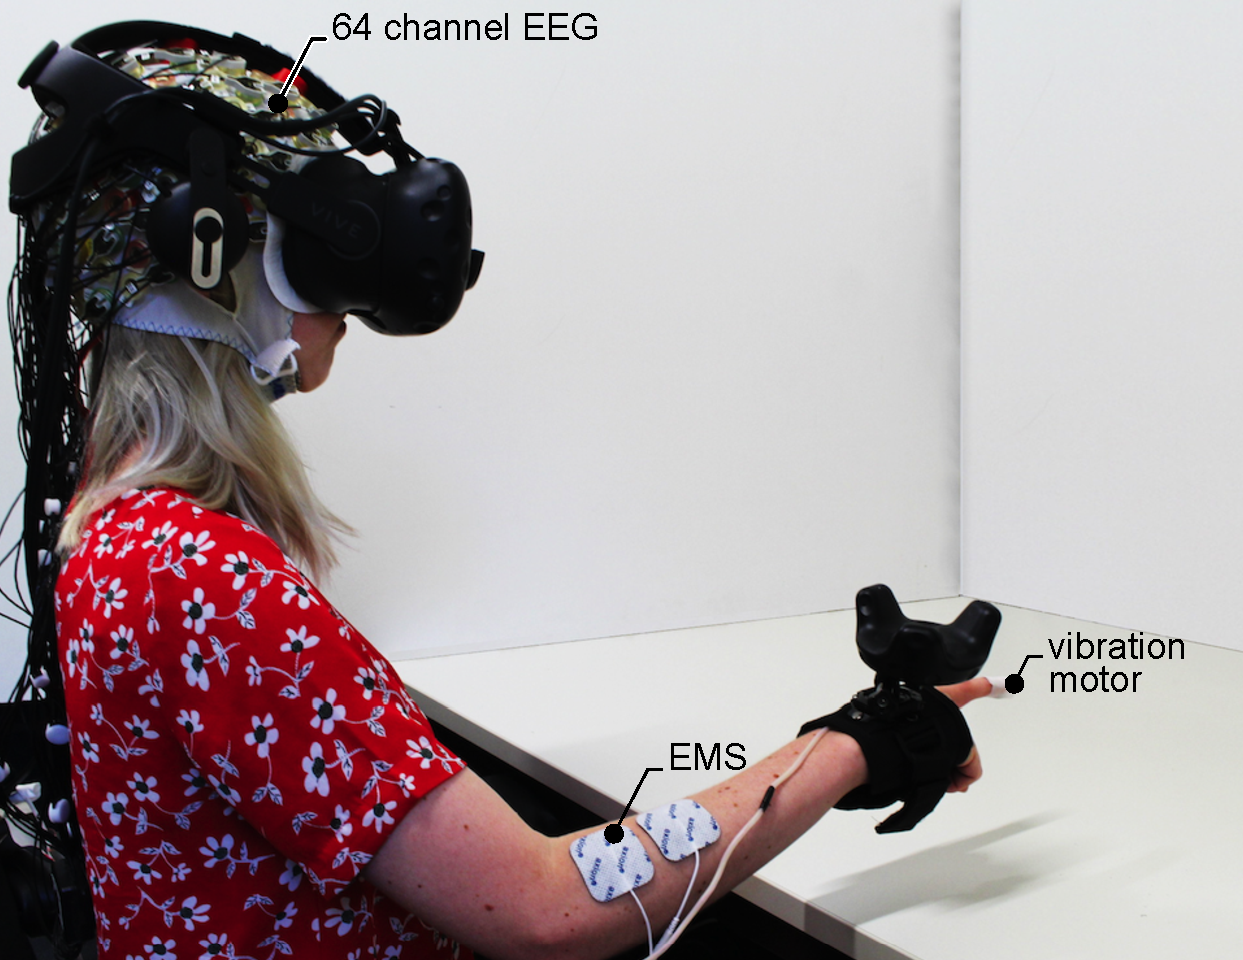
\includegraphics[width=\linewidth]{figures/experiment.pdf}
%\missingfigure[figcolor=white]{Shows setup.}
%\vspace{-17pt}
\caption{Our experimental setup (image with consent from participant).}
\label{setup}
\end{figure}

\textbf{(1) VR and hand tracking.} We used an HTC Vive headset (HTC Corporation, Taoyuan, Taiwan) with the Vive Deluxe Audio Strap and custem EEG cap spacers \footnote{https://grabcad.com/library/adapter-for-vr-eeg-setups-1} to ensure a good fit and less discomfort due to the EEG cap. We used a Vive Tracker, attached to the participant's wrist, to track their right hand. 

\textbf{(2) Vibrotactile feedback.} We used a vibration motor (Model \textit{308-100} from \textit{Precision Microdrives}), which generates 0.8g at 200Hz. This motor measures 8mm in diameter, making it ideal for the fingertip. The vibration feedback was driven at 70mA by a 2N7000 MOSFET, which was connected to an Arduino output pin at 3V.

\textbf{(3) Force feedback.} We actuated the index finger via electrical muscle stimulation (EMS), which was delivered via two electrodes attached to the participants' \textit{extensor digitorum} muscle. The finger actuation was achieved via a medically-compliant battery powered muscle stimulator (\textit{Rehastim} from \textit{Hasomed}), which provides a maximum of 100mA and is controllable via USB. 

% We utilized the extensor digitorum since we found that we can robustly actuate it without inducing parasitical motion of neighboring muscles; this was verified during pilot studies. This finger actuation was achieved via a medically-compliant battery powered muscle stimulator (\textit{Rehastim} from \textit{Hasomed}), which provides a maximum of 100mA and is controllable via USB. We chose this device since it had been successfully used by researchers as a means to generate force feedback in both VR~\cite{lopes_walls_2017} and AR~\cite{lopes_AR}. The EMS was pre-calibrated per participant to ensure a pain-free stimulation and robust actuation. 

\textbf{(4) EEG Setup.} EEG data was recorded from 64 actively amplified electrodes using BrainAmp DC amplifiers from BrainProducts. Electrodes were placed according to the extended 10\% system ~\cite{oostenveld_five_2001}. After fitting the cap, all electrodes were filled with conductive gel to ensure proper conductivity and electrode impedance was brought below 5kOhm for all electrodes. EEG data was recorded with a sampling rate of 1000 Hz. We synchronized tracking, EEG data, and an experiment marker stream that marked sections of the study procedure using labstreaminglayer\footnote{https://github.com/sccn/labstreaminglayer}.

\begin{figure*}[!ht]
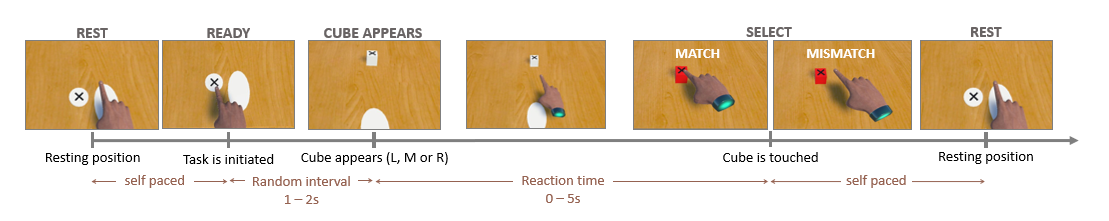
\includegraphics[width=\linewidth]{figures/Task_mismatch.PNG}
\vspace{-15pt}
\caption{Interaction flow depicting one trial in our 3D object selection task.}
\label{task_flow}
\end{figure*}

\subsection{Training phase}
We asked participants to wear the HTC VIVE VR headset for a maximum of 24 trials practice trials. Overall, the EEG fitting, calibration, and practice trials took around 30 minutes (with two experimenters).

\subsection{Task}
Participants performed a 3D object selection task in VR design with Unity Software (Unity Technologies, San Francisco, USA). The interaction flow of our task, depicted in Figure~\ref{task_flow}, was as follows: (1) participants moved their hands from the \textit{resting position} to the \textit{ready position}, to indicate they were ready to start the next trial; (2) participants waited for a new target to appear (the time of a new target spawning was randomized between 1-2 s); (3) then, the target (a cube) would appear in one of three possible positions (center, left, right), all equidistant from the participant's \textit{ready position}; (4) then, participants acquired the target by moving and touching the target with their index finger. (5) After a target was acquired, participants moved back to the \textit{resting position}. Here, they could take a break before the next trial.

\subsection{Interface conditions}
Participants performed the task in three additive feedback conditions:

(1) \textbf{visual-only (Visual)}: when participants touched the cube, it changed its color from white to red (visual feedback)
% ; our no-haptics \textbf{baseline}~\\
\indent(2) \textbf{tactile (Vibro)}: when participants touched the cube in the vibro condition, they received a 100 ms vibroactile stimulus and the color change (visual + tactile feedback)
% ; this is the only available haptic feedback in today's VR experiences.~\\
\indent(3) \textbf{force-feedback (EMS)}: in this condition, participants also received a 100 ms of EMS stimulation at the index finger extensor in addition to the visual and vibrotactile feedback (visual + tactile + force feedback)
% . As prior research showed the EMS stimulation of the opposing muscle (in our case, the extensor) is perceived as the resisting force that arises from pushing against the cube (i.e., force feedback)~\cite{lopes_muscle-propelled_2013,lopes_walls_2017,lopes_impacto:_2015}.

% We designed our three feedback conditions additively because additional haptic feedback is generally associated with more haptic realism, therefore, we hypothesized that ERPs would demonstrate some correlation to the ascending level of the feedback's realism.

\subsection{Introducing Visuo-Haptic Mismatches}
To allow us to compare the event-related EEG and movement signatures in a realistic vs. unrealistic interaction, we presented participants with two different classes of trials: \textbf{match trials (C)} (75\% of the trials) and \textbf{mismatch trials (M)} (25\%). This procedure elicits a prediction mismatch signal in 25\% of the trials similar to previous designs investigating the impact of target probabilities~\cite{polich_updating_2007}.  %on ERP modulations
In the \textbf{matching} trials, the feedback stimuli were presented upon touching the object, exactly when participants expected them to occur based on the available visual information (finger touching the target). In contrast, in the \textbf{mismatch} trials, the feedback stimuli were triggered prematurely, which was accomplished by enlarging the invisible radius of touch detection by 350\%. While in the match trials, we used a cube collider of the exact size of the VR cube, in the mismatch trials, we used a larger sphere collider. Our collider enlargement was based on the study design by Singh et al.~\cite{singh_visual_20008}, in which they showed that VR users can detect a visual mismatch at around 200\% of offset from the target. In our pilot tests, we decided to extend the offset to 350\% to make the mismatch more obvious so as to provoke more pronounced prediction errors. 

Also, we used a match-to-mismatch ratio of 75\%-25\% of the total trials by modeling our study after previous studies, which also ensure that participants are faced with a detectable unrealistic behavior of the virtual environment~\cite{Liao2011,Wiersema2007,Donchin1988}. For these unrealistic trials to occur, the participants must first be able create a stable model of how the VR world operates, thus the VR world cannot behave at a random 50\%-50\% match-mismatch ratio.

Finally, these match vs. mismatch trials were presented in five randomly generated sequences, each with an equal distribution of matches and mismatches.

\subsection{Experimental design}
The experiment consisted of five phases: (1) a setup phase; (2) a calibration phase; (3) a short training phase; (4) the task itself, in all three possible interface conditions, each followed by a subset of items from the IPQ questionnaire (G1, REAL2, SP4 and INV1)~\cite{T.W.Schubert2003} and the NASA-TLX~\cite{Hart1988}. Lastly (5) participants were asked about their experience in the VR and which condition they enjoyed the most.

% For completeness, at the end of each condition we presented the four most relevant questions from the standard IPQ~\cite{ipq_paper}, in particular: G1, REAL2, SP4 and INV1. However, our hypothesis was that the inclusion mismatch trials, which were presented in 25\% of the cases, would lower the IPQ ratings dramatically.

We used a within-subjects design with 300 trials for each, the Visual and Vibro feedback condition, and 100 trials for the EMS condition. The order of the Visual and Vibro conditions was randomized across participants with the EMS condition always being the last block. 
% This was done to avoid potential overshadowing of the EMS stimulation (a very strong sensation) on the two other stimulation conditions.





%%%%% resources:
% \subsection{Task and Procedure}
% Using an HTC Vive VR Headset with the Vive Deluxe Audio Strap and a Vive Tracker (HTC Corporation, Taoyuan, Taiwan) attached to the right hand, a 3D object selection task was presented on a virtual table placed on an infinite white plane. The virtual environment was created in the Unity3D engine (Version, company details). White cubes appeared at random either in the center, to the left, or to the right of the participant, equidistant from a starting position (see Figure ??). The time of a new cube spawning was randomized between 1-2 seconds after starting a trial. 

% %no subsections? This so hard to parse, make a task heading or so?
% Participants were tasked to select the cube with their index finger and, upon completion, move their hand back to a resting position indicated on the table. The task was completed in two blocks of 300 trials each, with one block providing visual-only feedback, i.e. the cube changing its color from white to red upon selecting, and one block providing visual-tactile feedback, in which the selection contact was indicated by the color change plus a small vibrotactile pulse. Placed under the index fingertip, a vibration motor (Model \textit{308-100} from \textit{Precision Microdrives}), generating 0.8g at 200Hz and measuring 8mm in diameter was driven at 70mA by a 2N7000 MOSFET connected to an Arduino output pin at 3V. An initial 24 trial training session was followed by the two experimental blocks (balanced across participants), each followed by two questionnaires, NASA-TLX and IPQ. For the main experimental manipulation of asynchrony, 25\% of the trials (totalling 75 asynchronous trials per feedback block of 300 trials) exhibited spatio-temporal asynchrony in line with established oddball paradigms. Object selection was triggered prematurely by bounding a spherical collider to the cube and enlarging it by 350\% in comparison to a collider bounded to the shape of the cube in the synchronous trials. Asynchronous trials were sorted in a pseudo-randomized sequence following synchronous trials, i.e. between one and five synchronous trials preceeded an asynchronous trial. Extended task and apparatus descriptions can be found elsewhere \cite{Gehrke2019}.
% % todo add movie, figure and references
\subsection{Data acquisition}

EEG and mocap here
%todo
% how many channels were removed on average?
% what where the ICLabel settings for cleaning?
% update with standard text of bemobil pipeline
\subsubsection{EEG-recording and pre-processing}

\begin{comment}
EEG-data was recorded from 64 active electrodes with a sampling rate of 500 Hz (Brainproducts GmbH, Gilching, Germany). Electrodes were mounted on an elastic cap (cite here: EASYCAP, Herrsching, Germany) with placing according to the extended international 10–20 system \cite{chatrian_ten_1985}. The electrode at position FP2 was detached from the cap and placed under the left eye, in order to measure participants Electrooculogram (EOG). Impedances were kept under 30 \si{\kohm}.The data preprocessing and analysis were performed in Matlab 2017  (MATLAB, The MathWorks Inc., Natick, MA, USA), using the EEGLAB toolbox \cite{delorme_eeglab:_2004} and the 'BeMoBIL Pipeline' \cite{klug2018bemobil} plugin. The single subject data was lowpass filtered with 124Hz and down-sampled to 250Hz. Channels which were contaminated with artifacts were automatically rejected using the PREP pipeline \cite{bigdely-shamlo_prep_2015} 'FindNoisyChannel' function, which is selecting bad channels by amplitude, the signal to noise ratio and correlation with other channels. Rejected channels were then interpolated while ignoring the EOG channel, and finally re-referenced to average reference (data A).
The data was then filtered with a 1 Hz highpassfilter (data B), a first adaptive mixture independent component analysis, AMICA \cite{palmer_newton_2008}, was used to identify eye related independent components (ICs) which were projected out of the sensor data (data A). For this, the rank was reduced by one for average reference use and further, the number of interpolated channels in the respective data set. To identify eye components IClabel  \cite{pion2019iclabel} was used, whereas components exceeding a value of 0.7 for the 'eye' class were defined as eye components.
Then, to detect segments of noisy data, an automated time domain cleaning (see \citet{gramann2018heading}) on the time domain was performed on narrowly filtered data from 1 to 40 Hz. The data was therefore first split into 1 second long segments for which the mean absolute amplitude and standard deviation of all channels as well as the Mahalanobis distance of all channel mean amplitudes were calculated. All three methods results were then joined together in order to rank all segments. The 12\% highest ranking noisy segments were selected for rejection and an additional buffer of +/- 0.49 sec was added around each segment resulting in about 15\% rejected data for each subject. This data was rejected from data B and a second AMICA was calculated on this time domain cleaned data. A dipole fitting \cite{oostenveld2002validating} was performed for each spatial filter and the spatial filter information was then copied back to the preprocessed, interpolated and average referenced data set (data A).
To study event-related potentials, a 0.1 Hz to 40 Hz filter was applied  and eye components as well as line noise components were projected out, again with component labeling using ICLabel (both thresholds set to 0.8). The continuous data streams were then epoched from 1200 ms pre-target stimuls (200ms before reference stimulus) to 1200 ms post-target stimulus presentation. Automatic epoch cleaning was applied using the same procedure as described above, rejecting 10\% of the noisiest epochs.
All epochs containing mismatch trials, incorrect responses, as well as reaction times exceeding two standard deviations (sd) from participants mean reaction time in the respective difficulty level, were excluded from further analysis on EEG and behavioral level. The same procedures were applied to create longer epochs up to 6000 ms post-target stimulus in order to properly plot the ERP Image \cite{delorme2015grand} sorted by reaction times. (check number of remaining trials etc and add here)
%check number of remaining trials etc and add here
\end{comment}

Artifactual channels were manually identified, removed, and interpolated using spherical interpolation (on average, X channels were interpolated, SD=Y). Subsequently, the data was re-referenced to the average of all channels and a zero-phase Hamming windowed high-pass FIR filter (order 827, pass-band edge 1 Hz) was applied to the data. Concatenated data from all individual explorations was parsed into maximally independent components (IC) using the adaptive mixture of independent component analyzers (AMICA) algorithm with prior principal component analysis (PCA) reduction to the remaining rank after interpolation\citep{Palmer2011}. Subsequently, independent components reflecting eye activity were subtracted from the data in order for an automated cleaning procedure across channels in the time domain not to be affected by eye signals. All Components were automatically matched against the ‘ICLabel’ database and components with a probability >= .XY to reflect eye activity were subtracted\citep{iclabel}. Subsequently, 15\% of the noisiest time segments were determined by jointly ranking the amplitude mean, standard deviation, and mahalanobis distance across channels of consecutive one-second epochs\citep{cleaning_fh2018}. Subsequently, artifactual time windows were rejected from the concatenated data prior to eye component removal and a second ICA was computed on this cleaned data containing eye movement signals. Hence in a first step eye movement components were rejected to subsequently find noisy segments in the data not related to eye movements.

For each IC, an equivalent dipole model was computed as implemented by DIPFIT routines in EEGLAB. Using the 10-20 standard electrode locations, a a boundary element head model (BEM) based on the MNI brain (Montreal Neurological Institute, MNI, Montreal, QC, Canada) was used with DIPFIT routines. We refer to the approximated spatial origin of an IC as “in or near” a specified location.

\subsubsection{Group-level analyses: Clustering}
% todo
% ICLabel settings selecting components
To allow for group-level comparisons of EEG data at the source level (ICs), components with a probability of XY using ICLabel were selected and subsequently clustered based on their equivalent dipole locations (weight=6), grand-average ERSPs (weight=3), mean log spectra (weight=1), and scalp topography (weight=1), using a region of interest (ROI) driven repetitive k-means clustering approach\citep{cleaning_FH2018}. The weighted IC measures were summed and compressed using PCA, resulting in a 10-dimensional feature vector for clustering. ICs were clustered by applying the k-means algorithm with k equaling 70\% of the mean number of ICs retained across subjects. We chose to use fewer clusters than ICs per participant because of our assumption that, although statistically independent per time point, there may be more than one IC per participant that is similar in function and location. ICs with a distance of more than three standard deviations from any final centroid mean were considered outliers.

% todo: update with final clustering solution properties
To ensure replicability of the clustering, we employed the same clustering approach reported in\cite{cleaning_FH2018}. After applying desirable weights (number of participants: 3, ICs/participants: -1, spread: -1, RV: -1, distance from ROI: -2, Mahalanobis distance from the median: -1) the final clustering solution contained the ICs from 25 participants, a ratio of 1.13 ICs per participant (two participants with two ICs each), a spread of 296, a mean RV of 10.3\%, and a distance of 10.2 units in the Talairach space for the cluster of primary interest.
%averaging of ICs → citation why that is either okay (Delorme?) or problematic :), one reason why doing this makes sense is to avoid higher weighting of individual subjects based on more ICs per cluster.
\subsubsection{Group-level analyses: Statistical parametric spectra and time-frequency maps}
Spectra and event-related spectral perturbations (ERSP\citep{Makeig2004}) were analyzed on the group level using robust repeated-measures ANOVA\citep{Pernet2011} to test for the effect of repetition and multiple regressions to assess the influence of each behavioral parameter individually. Initially, we obtained estimates of each subjects response by mass-univariate modeling of each ERSP time-frequency point. We fitted the model $Y = Maze*Repetition + Touch_Duration$ to control for the effect of touch duration. Since allowing continuous interaction with the touchable walls introduced the confound of touches/epochs of different duration. The resulting regression estimates (Betas) were used as each single-subjects summary for group-level inferences.

To characterize the mapping between event-related brain dynamics and the stimulus properties of the time-locked events we employed a hierarchical linear modeling approach on the time-frequency data. First, single-trial regressions weights were estimated for the factors maze and trial run, their interaction, as well as a continuous noise predictor (touch duration “slope rERSP”) for each time-frequency pixel across trials [Rousselet 2008,2009,2010]. We chose a resolution of 96 frequencies  (~3 to ~100 Hz) and 177 timepoints (-300ms to 714ms) around the wall touch event. Since single trials were warped linearly to the same length we corrected for the warping by regressing the touch duration (see above) on each time-frequency pixel across single trials. Before regression, touch duration was centered on 0. Hence, estimates for the categorical predictors are interpreted when touch duration is at its mean value. After adding back the intercept and summing across the corresponding regression terms for each of the 12 factor levels (3 Maze Trials X 4 Mazes), single trial estimates were averaged (in power) for each factor level. Whole epoch average power per factor level was then baseline corrected using a divisive baseline, i.e. mean power values in each frequency across the -300 to -100ms window pre wall touch. Subsequently, power values were transformed to the decibel scale using 10 * log10 (factor level average baseline corrected power).

Using LIMO EEG, subject estimates from the first level were taken as input for group level inference testing [Pernet2011,Rousselet2011,Cohen2011]. To investigate the main effect of both factors, run and maze, we computed 3 (Runs) X 4 (Maze) repeated-measures ANOVAs for each time-frequency pixel for each IC k-means cluster independently. We addressed the multiple comparison problem by correcting the FWER using the threshold-free cluster-enhancement statistic (TFCE, [cite smith and nicols, 2014]). TFCE statistical maps were computed for each of 1000 bootstraps obtained by sampling with replacement across participants. A distribution of maximum TFCE scores was build, keeping the max TFCE score per bootstrapped time-frequency map. The TFCE scores of the true result were then thresholded with the 0.95 percentile (alpha = 0.05) score of the max TFCE distribution.

In order to investigate the relationship between ERSPs and parameters of spatial learning, we build a regression model using group level data as input. Taking factor level data as the dependent variable, we entered both sketchmap scores and exploration duration as continuous predictors, assuming a continuum of a mental spatial representation represented by discrete sketchmap scores. For simplicity, we did not consider any interaction terms with the experimental design (3 maze trials X 4 maze). As above, to correct for multiple comparisons, TFCE scores of bootstrapped samples were used to build a max TFCE distribution to determine the alpha level threshold value.

For visualization purposes, group average ERSPs were obtained by averaging dB time-frequency maps significance masked by threshold surviving TFCE scores.
% end clean up
\subsection{Modeling the impact of haptics}

\section{Results}

\subsection{Clustering and Localization of Independent EEG Sources}
Several independent component (IC) source clusters showed event-related changes in power. The numbers of subjects contained in each cluster as well as Tailarach coordinates of the cluster centroids are given in \ref{fig:localization}.

\begin{table}
\caption{\label{tab:}IC clusters and cluster centroid locations}
\centering
\begin{tabular}[t]{l|r|r|l|l}
\hline
Talairach coordinates & Nr. of subjects & Cluster & Cortical location & Brodmann area\\
\hline
-6, -83, 20 & 22 & 6 & Occipital & BA18\\
\hline
39, -66, 27 & 24 & 13 & Right temporal/parietal & BA39\\
\hline
2, 9, 37 & 19 & 15 & Anterior cingulate & BA32\\
\hline
-34, -35, 43 & 16 & 20 & Left parietal & BA40\\
\hline
-1, -53, 22 & 25 & 25 & Posterior cingulate / RSC & BA23\\
\hline
\end{tabular}
\end{table}

%\input{figures/source_localization.tex}
\section{Discussion}% start with summary
% aim for 1500 - 2000 words

% Points to discuss
% - is classification success dependent on level of haptic immersion? -> cite that it also works better in meditators for example

Coherent multisensory integration yields meaningful perceptual experiences and is central to adaptive behavior because it allows animals to perceive a world of coherent perceptual entities. In this work, we present evidence for neural signatures originating in central-parietal EEG sources during a spatio-temporal multisensory binding challenge. In order to carve out a signal separating cases of spatio-temporal synchrony from asynchronous cases we employed brain-computer interface technology. Through localization of the classifier weights we gained access to a node in the hierarchical inference network. Subsequent single-trial analysis on the spectral signatures exhibited a separation of alpha- and theta-band characteristics. In the time-domain, the signature can be employed for human-computer interaction purposes as we have shown it is accurately classifiable in two classes. Further, we functionally distinguished theta-band activity from alpha-band activity using single-trial regression. Alpha-band activity following spatio-temporal asynchrony was predicted by baseline activity as well as reaction time, the time elapsed to reach for the target. Both predictors allude to the general temporal task structure and hence may be separated from instantaneous processing. On the other hand, theta-band burst succeeding a binding challenge referred to the multisensory context, that is rendered physics and its interaction with the instantaneous hand velocity.


% maube good conclusion?
Adding to the significant body of evidence about (bayesian) prediction error computations, our findings enable targeted signal acquisition for neural interface technology in VR. 


%%%% writing ressources below
% - discuss reasons for low R^2 and approaches to address it (experiment design and methods (unfolding other processes, adding regressors etc.)) is there a meta study on effect sizes in timefrequency resolved EEG studies. What does Johanna report, regarding effect size?
% - is proprioceptive feedback important in our task: I'd argue against that because I consider vibration on the fingertip to be an exteroceptive sensation and do not consider it relevant where the hand was and how my joints were angled etc. during the mismatch event, therefore i stick to exteroceptive prediction errors only!
% - On world stability: designing visuo-haptic mismatches in virtual environments means further complicating the action-perception cycle understood as hypothesis testing. By pseudo-randomizing when one of the 25 percent chance oddballs appears, hypothesis testing and subsequent evaluation of the latent variables causing the oddball to appear becomes meaningless.

% then summarize results as below paper claim:
%(touch epochs)
%1. LDA location: Central-parietal EEG source activity discriminates between predicted and perturbed visuo-haptic perceptual experiences, in our case the touching of a cube on a desk, baring similarities to a classical simon task.
%(full epochs)
%2.1. ICs clustered to the centroid of the weighted ICs contributing the strongest to the LDA classifier were located to an area between precuneus and posterior cingulate cortex.
%2.2. Hand velocity characteristics, an event-related potential as well as an event-related spectral signature were explained by adding a haptic channel, increasing the level of immersion in the perceptual experience.
%2.3. Further, we observed responses locked to the feedback onset independent of differences in ongoing motor behavior between matching and mismatching classes. (description-level)
%(touch epochs)
%3.1. IC source dynamics following a visuo-haptic perturbation differ from predicted perceptual experiences (see 1., show difference erp and ersp)
%3.2. Following a visuo-haptic perturbation, the context of said perturbation operationalized by hand velocity, haptic feedback and their interaction, impact IC source dynamics only faintly.
%(next trial epochs)
%4. Post perturbation behavioral adaptation is in line with previous findings and may be explainable through reinforcement learning like computations in the brain.

% 1. start with a summary of the most important results
% -> what was the goal of this research?
% 2. situate findings in literature
% -> challenges for mobi research and how to make stimuli more salient
% -> bodily self perception
% 3. link back to introduction and papers cited in introduction

%so there are 2 things participants do in the task: 
%1. they collide too early and immediately adapt hand movement and have mmn / frontal theta -> Prediction Error
%2. they do RL using PE signal and adapt subsequent behavior (trial after mismatch)

% some arguments why ERP:
% - see Cohen 2014 muscle twitches: In our final set of analyses,we examined the ERPs—the time-domain EMG onset-locked EEG potential. Thiswas done mainly to replicate previous findings concerning the relationship between the ERP and partial errors.
% - moving towards an applicable metric to detect things online, hence must be computationally inexpensive, therefore ERPs
% - use ERP section as exemplary for understanding results
% - In haptically richer environments, processing gets more accurate and hence amplifies the error signal originating in or near anterior cingulate cortex (ACC). Moving fast and experiencing richer haptic feedback impact error processing
% - how does erp and ersp correlate. gamma and n200 occipital etc. filtering low frequency for erp does not mean higher ERSP frequency burst might not add to slow cortical ERPs -> therefore, approach is valid

% - discuss with spatial conflict processing: Savoie, & Simon Task results: cohen, cavanagh, toellner
% - reference to self and body ownership, spatial computations between egocentric and allocentric? cite Ehrsson, Slater, Gonzales-Franco (uncanny valley of haptics)
% - single-trial regression challenges in mobile brain body imaging studies: energy of stimulus, Time-locked vs. continuous regressors/stimuli, EEG artifacts due to movement, Contrast desktop stimulation vs. wide FOV in VR, Higher cortical noise, Saliency of stimulus, necessary attention on stimulus %in terms of predictive coding,
% - Study specific shortcomings: low N, both in subjects and in trials due to oddball paradigm
% - assume frontal evaluation of asynchronoy guiding future action and therefore did bot correlate any EEG metric with a post-error slowing parameter.
% - IC sources located near posterior cingulate cortex may anchor the self in the afforded reference frame, providing grounds for spatial predictions during ongoing perceptual experience.


% Submissions are not required to reflect the precise reference formatting of the journal (use of italics, bold etc.), however it is important that all key elements of each reference are included.
\bibliography{references}

\end{document}
